

%\documentclass[aps,pra,onecolumn,tightenlines,floats,superscriptaddress,11pt]{revtex4}
\documentclass[12pt,a4paper% die Verwendung von DIN-A4-Format ist pflicht!
]{article}
 \usepackage[top=3cm, bottom=2.5cm, left=2cm, right=2cm]{geometry}
% 
% %notwendige Pakete
 \usepackage[english]{babel}    % mehrsprachiger Textsatz
% babel: letzte Sprache in Optionen zeigt die Sprache des Dokumentes
% und kann durch den Befehl \selectlanguage{} geaendert werden
% Passen Sie die Optionen des babel-Paketes nach Bedarf an!
\usepackage[latin1]{inputenc}       % Eingabekodierung Parameter latin1 darf ge�ndert werden
\usepackage[T1]{fontenc}                % Schriftenkodierung
\usepackage{graphicx}                       % zum Einbinden von Grafiken
\usepackage{lmodern}                        % Ersatz fuer Computer Modern-Schriften
                                                                % zum besseren Aussehen am Bildschirm
\usepackage{amssymb} 
 \usepackage{amsmath} 
 \usepackage{float}
 \usepackage{listings}
 \lstset{breaklines = true}
 \usepackage{fancyhdr}
 \usepackage{url}
 \usepackage{pdfpages} 
 \setlength\parindent{0pt}
 %\usepackage{subfigure}
 \usepackage{color}
 \usepackage{tabularx}
 \usepackage{chemfig}
 \usepackage{braket}
 \usepackage{multirow}
\usepackage{bigdelim}
\usepackage{caption}
\usepackage{subcaption}
\usepackage{flafter}
 \usepackage{bbold}
\usepackage{calligra}



 \newcommand{\fe}{\textbf}
 \newcommand{\om}{\omega}

 \newcommand{\up}{\uparrow}
 \newcommand{\uu}{\up\, \up}
 \newcommand{\down}{\downarrow}
 \newcommand{\dd}{\downarrow\, \downarrow}
 \newcommand{\halb}{\frac{1}{2}}
 \newcommand{\half}{\frac{1}{2}}
  \newcommand{\tspace}{\rule{0pt}{2.6ex}}
  \newcommand{\norml}{\textnormal}
  \newcommand{\op}[1]{\mathrm{\hat{#1}}}
  \newcommand{\summigral}{\int\!\!\!\!\!\!\!\!\!\;\sum}
  \newcommand{\tr}{\mbox{tr}}
 \newcommand{\pardiff}{\frac{\partial}{\partial t}}
 \newcommand {\cphi}{\cos\left(\frac{\varphi}{2}\right)}
 \newcommand {\cthe}{\cos\left(\frac{\theta}{2}\right)}
 \newcommand {\sphi}{\sin\left(\frac{\varphi}{2}\right)}
 \newcommand {\sthe}{\sin\left(\frac{\theta}{2}\right)}
  \newcommand {\cn}{\norml{c}}
    \newcommand {\sn}{\norml{s}}
    
\def\beq{\begin{equation}}
\def\eeq{\end{equation}}
\def\beqa{\begin{eqnarray}}
\def\eeqa{\end{eqnarray}}    
 \newcommand{\blue}[1]{\textcolor{blue}{#1}}  
 
 
\begin{document}
\section{Introduction}


\section{Facilitation condition and synthetic Lieb lattice}
%
We consider a quasi one-dimensional array of optical tweezers, each loaded with a single Rydberg atom.
Our system is extended in the $x_1$ direction and restricted to two layers in the $x_2$ direction, forming a Rydberg ladder.
The atoms are described as effective two-level systems with the electronic ground state $\ket{\up}$ and the excited Rydberg 
state $\ket{\down}$. 
The separation of the atoms in the optical traps $R_0$ is equal in both directions of the ladder $\{x_1,x_2\}$.
The Rydberg lattice system is described by the Hamiltonian (in  rotating wave approximation)
%
\begin{align}
 \op{H} = \Omega \, \sum_k^N  \op{\sigma}_x^{(k)} \, + \, \Delta\, \sum_k^N\,\op{n}_k +\, V_0 \,
 \sum_{\substack{k= 1\\ m \ne k}}^N \, \frac{\op{n}_m\, \op{n}_k}{|k -m|^\gamma},
 \label{Eq:Hamil_full}
\end{align}
%
where $\Delta$ is the detuning, $V_0$ is the coupling strength and $|k -m|$ gives the distance between
the atoms located at site $k$ and $m$.
%
%
\subsubsection{disorder coupling of channels by disorder and beyond + properties of fat-tail distribution: correlated, diverging moments}

For small temperatures $T$ the atomic position in the trap can be approximation by a Gaussian distribution Eq. \eqref{Eq:Gaussian_distribution} with width $\sigma$.
This results in a fat-tail distribution of the interaction displacement $\delta V$.
In the case of two Rydberg atoms with $\delta v =\delta V/V_0 $ and $s = \sigma/R_0$ it is given by
%
\begin{align}
 \mathcal P_2 (\delta v |s) =
 \frac{1}{\alpha \sqrt{\pi}\, s\, ( 1 + \delta v )^{1+\frac{2}{\alpha}}} 
\text{e}^{-\frac{1}{4 s^2}\left[ 1+(1+\delta v)^{-\frac{2}{\alpha}}\right]}
\sinh\left(\frac{1}{2s^2}(1+\delta v)^{-\frac{1}{\alpha}}\right)
\label{eq:fattail}
\end{align}
%
The fat-tail distribution $\mathcal P_2 (\delta v |s)$ has diverging moments and yields correlated $\delta_v$.
%
Note, the disorder acts in a Rydberg lattice only on the intermediate lattice sites corresponding to neighboring Rydberg excitations.
Hence, only intermediate lattice sites experience the disorder while the main sites are unaffected.
We refer to this kind of correlated disorder as ``experimental 
disorder''.
%
\subsubsection{facilitation condition + discuss exponents}
\begin{figure}
% 	    

	      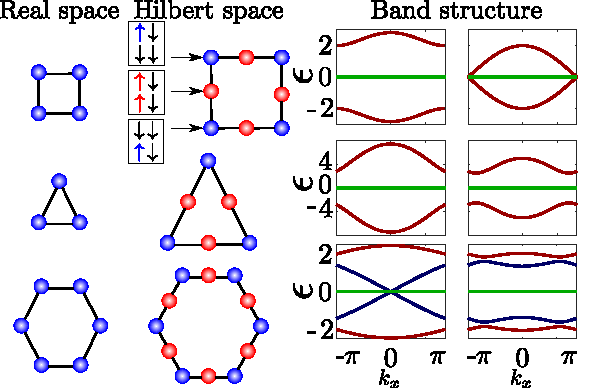
\includegraphics[width=0.5\textwidth]{graphics/lattices_real_hilbert_bands.pdf}

    %
		\caption{
		    First column: geometry of a square, a triangular, and a hexagonal lattice 
		    in real space. The blue spheres give the position of the Rydberg atoms and
		    the lines the interaction between neighboring atoms. Second column: respective lattices in Hilbert 
		    (for $\Delta = -V_{NN}$). The blue dots represent the main state with a single excitation while the red spheres
		    are intermediate state corresponding to a single pair of neighboring excitation.
		    Third column: two cuts of the band structure for each lattice geometries at $k_y= 0$ (left) and $k_y = \pi$ (right).
		    The green bands are the flat bands of the respective lattice. The red and blue bands are the dispersive bands of the system
		    (different colors for easier readability).
		    %
                    }
  
	\label{Fig:flat_band_lattices}
\end{figure} 

%%
%%
%%
We consider the system under the anti-blockade ('facilitation') condition ($\Delta = -V_{\text{NN}}$), where 
the excitation of an atom to a Rydberg state is strongly enhanced by an excited neighbor. 
The facilitation radius coincides with the lattice spacing $R_0$. 
To describe the facilitated dynamics of the system, we assume $\Delta = -V_{\text{NN}}~\gg~\Omega$ 
leading to a strong suppression of unfacilitated transitions.
Consequently, spins are only allowed to flip if they have exactly one excited neighbor.
Furthermore, $V_{\text{NNN}}~\gg~\Omega$ which 
prohibits a spin flip next to two neighboring excitations.
Under these conditions, the number of excitation clusters $N_{cl}$
and the number of excitation triplets $N_{\text{NNN}}$ is conserved.
The second requirement contains $V_{\sqrt{2\text{NN}}}~\gg~\Omega$, which prevents the
excitation diagonal spins.
These requirements result in the truncation of the Hilbert space neglecting the possibility of having more than
two neighboring excitations simultaneously, and restricting the interaction to nearest neighbors (further details \cite{a_Marcuzzi_PRL_17}).

%
%
%
\subsubsection{synthetic lattice and flat bands + generalization to different geometries}
%
%
Due to the restriction of the Hilbert space, our system lives on a sublattice with $N$ single excitations, where $N$ is the number of lattice sites, and 
$M$ states with a single pair of excitations, where $M$ coincides with the number of bonds in the lattice.
We denote the former states as the $main$ states
(blue spheres), while
the latter states are the $intermediate$ states (red spheres). 
Figure \ref{Fig:flat_band_lattices} shows the occurrence of flat bands in Rydberg lattices of various geometries under the facilitation condition.
%
%
A Lieb lattices is a system with a macroscopically degenerate flat band formed by localized eigenstates with zero energy. 
In systems with flat dispersion bands, compact localized eigenstates (CLS) \cite{a_Leykam_EPJB} can occur which are in our case characterized 
by a non-zero amplitude on the intermediate sites of a single plaquette. 

The 1D-Lieb lattice (Lieb ladder) supports a flat band (FB) $ E_\norml{FB} = 0$ and four dispersive bands given by
% 
$\epsilon(k)  = \left\{\pm 2\cos\left(\frac{a\,k}{2}\right), \pm \sqrt{4+2 \cos(a\, k)}\right\}$\, in Figure ~\ref{Fig:decoupling}(d).
%
%
%
\subsubsection{two channels}
%
%
Note, the Lieb lattice decouples into two sublattices \cite{a_Flach_EPL_14,a_Leykam_EPJB}, a stub lattice and an ordinary 1D chain as shown in Figure \ref{Fig:decoupling}(c,d).
This results in two transmission channels $(X_n^-,Y_n^-)$ and $(X_n^+,Y_n^+)$, where each channel is described by a distinct localization length.
Introducing a small disorder of strength $W$ to the system, coupling the localized with the dispersive bands, lifts the degeneracy of the flat band and thus
the localization of the CLS.
%
%---------------------------------------------------------------------------------------------------------------------------------------------------------------------------------------
\section{Lieb ladder with correlated disorder}
%
\begin{figure}
% 	    

	      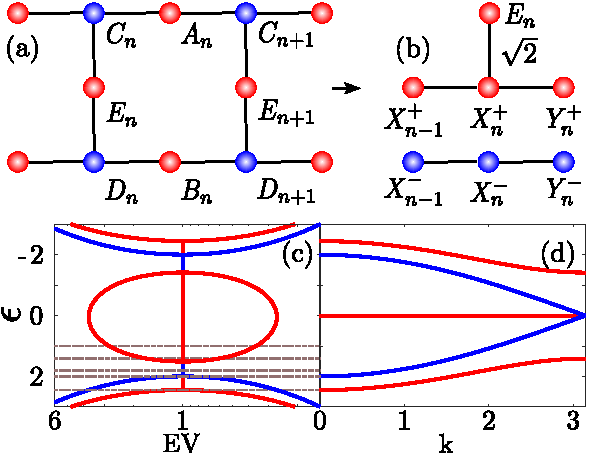
\includegraphics[width=0.5\textwidth]{graphics/decoupling.pdf}

    %
		\caption{(a) One dimensional Lieb ladder. Blue spheres correspond to the main states (singly excited states) and red spheres represent intermediate state
		(doubly excited states). (b) Lieb lattice after the detangling procedure introduced in \cite{a_Flach_EPL_14,a_Leykam_EPJB}.
		     (c) Eigenvalues of the transfer matrix in the case of no disorder.
		     The dotted lines corresponds to the energies $\epsilon = \{0,1, \sqrt 2, 1.8, 2, \sqrt 6\}$ at which the scaling of the localization lengths is determined.
                    (d) Band structure of the Lieb ladder without disorder. The bands corresponding to the stub lattice are given in red and bands of the ordinary 1D chain are shown in blue.
                    }
  
	\label{Fig:decoupling}
\end{figure}  
%
%
\subsubsection{Transfer matrix}
%
We explore the influence of the disorder on the localization behavior of the 
the Lieb ladder. A measure of localization is the localization length $\xi$ which defines the exponential decay of the eigenstate $\propto \text{e}^{1/\xi}$ \cite{a_Kramer_RPP_93}.
The localization length $\xi$ can be identified as the inverse of the Lyapunov exponent $\gamma$, which we obtain with the transfer matrix formalism \cite{b:Crisanti}.
The transfer matrix of the system in the $XY$ basis is
%
  \begin{align}
    \op{T}_{XY} = 
    \begin{pmatrix} 
	\gamma \alpha + \delta_{Y^-} \delta_{X^-} -1        &   \gamma \delta_{X^-} -\alpha \delta_{Y^-}               & -\gamma         & \delta_{Y^-}\\
	  -\beta \delta_{X^-} - \alpha \delta_{Y^-}         & \beta \alpha + \delta_{Y^-} \delta_{X^-} -1              & \delta_{Y^-}      & -\beta \\
	  \epsilon - \delta_{X^+}                                & -\delta_{X^-}                                          & -1              & 0\\
	    -\delta_{X^-}                                 &  \epsilon-\delta_{X^+}                                        &  0              & -1        
  \end{pmatrix}
  \label{Eq:Transfer_Matrix}
  \end{align}
 where $\gamma = \epsilon -\delta_{Y^+} - \tfrac{2}{\epsilon-\delta_E}$, $\alpha = \epsilon - \delta_{X^+}$, and $\beta = \epsilon - \delta_{Y^+}$.
 In the case of a 1D Lieb lattice with two significant Lyapunov exponents, it is straightforward to derive the transfer matrix in the decoupled $\{X_i,Y_i\}$ basis 
 while the derivation in the original basis has to be performed according to \cite{a_Dwivedi_PRB_93}. 
 than in the original
 basis.
%
$T_{XY}$ is a symplectic matrix with determinant one. 
The eigenvalues (EV) for zero energy and a disorder only acting on intermediate site are
 $\text{EV} = \left\{-1,-1, \lambda, 1/\lambda\right\}$ with $\lambda =  -\tfrac{\delta_E + \delta_{X^+} + \sqrt{\delta_{X^+}
 (2 \delta_E + \delta_{X^+})}}{\delta_E}$.
%

%
%



\subsubsection{localization length as function of s}

In the Lieb lattice, we can construct a non-localized zero energy state which is extended over the whole lattice. 
This state has non-zero contributions on all main lattice sites of the system, 
which are, as already mentioned, not effected by disorder. 
Because of this, the second Lyapunov exponent for $\epsilon = 0$ must be zero resulting in an exponential scaling of the 
localization length $\xi_2$ with system size $N$. The localization length $\xi_2$ at zero energy becomes independent of the disorder strength. 
This can be explained by the symplectic nature of the transfer matrix.\\
%
%%
Figure \ref{Fig:2D_loc_length}(a) shows the localization lengths $\xi_1$ and $\xi_2$ as a function of the energy $\epsilon$ and the disorder strength $s$ for 
the experimental disorder and dipole-dipole interaction $\alpha = 3$. 
The two channels described by $\xi_1$ and $\xi_2$ show a different localization behavior
leading to different speeds for the excitation transport in the two channels.
We can connect the spectra of the localization length $\xi_1,\,\xi_2$ with the eigenvalue spectrum of the transfer matrix Figure \ref{Fig:decoupling}(c).
The solid lines in Figure correspond to the dotted lines in the eigenvalues of the transfer matrix.
We find that the delocalized region in Figure \ref{Fig:2D_loc_length}(a) at $\epsilon \in \{\sqrt 2,2\}$
corresponds to the blue part in the eigenvalue spectrum of the transfer matrix.
However, the behavior of $\xi_2$ coincides with the red part in the eigenvalue spectrum in Figure \ref{Fig:decoupling}(c).
We observe a ``bending'' of the of the delocalized region of $\xi_1$ (Figure \ref{Fig:2D_loc_length}(a)) towards higher energies $\epsilon>2$, which does not occur for flat disorder.
This bending is caused by the increase of the parameter $s$, which increases the disorder strength and changes the band structure of the disorder-free problem.





\begin{figure}

	      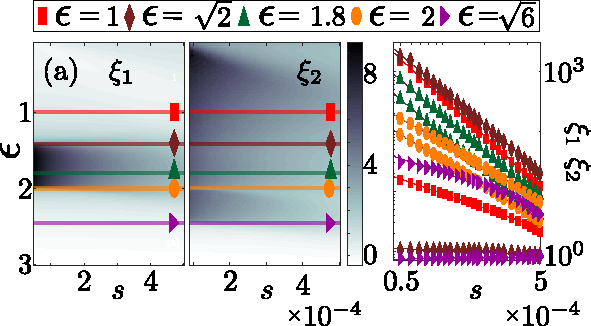
\includegraphics[width=0.5\textwidth]{graphics/loc_length_dipole_BW.pdf}

    \caption{(a) Localization lengths $\xi_1,\,\xi_2$ (color code)  as a function of the energy $\epsilon$ and the disorder strength $s$.
              The localization lengths along each of the black lines are shown in (b).
              The power law exponents $\nu$ of $\xi_1,\,\xi_2$ are
                $\nu\left(\epsilon = 1\right)$ = \{ 0.1006~$\pm$~0.004, 1.96~$\pm$~0.03\}, 
 	        $\nu\left(\epsilon = \sqrt{2}\right)$ = \{ 0.823~$\pm$~0.006, 2.16~$\pm$~0.06\},
 		$\nu\left(\epsilon = 1.8\right)$ = \{ 1.986~$\pm$~0.007, 2.01~$\pm$~0.01\},   
  		$\nu\left(\epsilon = 2\right)$ = \{ 1.428~$\pm$~0.007, 1.376~$\pm$~0.007 \},
 		$\nu\left(\epsilon = \sqrt{6}\right)$ = \{ 0.034~$\pm$~0.002, 0.79~$\pm$~0.01 \}.
	 The atomic position distribution is a Gaussian with width $\sigma$, and the interatomic interaction is a dipole-dipole interaction ($\alpha = 3$) with an interaction strength of $V_0 = 300$.
	     } 
   \label{Fig:2D_loc_length}
\end{figure}  



\subsubsection{discuss ``anomalous'' scaling presumably caused by correlations in disorder}
Reference \cite{a_Leykam_EPJB} gives the power law exponents for various energies
%
\footnote{Power law exponents \cite{a_Leykam_EPJB}:
$
E = 1:\{\nu_{\xi_1} = 0,\nu_{\xi_2} = 2\}, E = \sqrt 2:\{\nu_{\xi_1} = 2/3,\nu_{\xi_2} = 4/3\},E = 1.8:\{\nu_{\xi_1} = 2,\nu_{\xi_2} = 2\},
E = 2:\{\nu_{\xi_1} = 2/3,\nu_{\xi_2} = 4/3,E = \sqrt 6:\{\nu_{\xi_1} = 0,\nu_{\xi_2} = 2/3\}\}
$.}
for a Lieb ladder with a flat disorder 
potential acting on all lattice sites, which we can reproduce in our setup where the (flat) disorder only acts on intermediate lattice sites.
%
When we apply the experimental disorder to our system, we find an anomalous scaling behavior of the localization lengths
shown in Figure for $E = \sqrt{2}, 2$. In Fig \ref{Fig:2D_loc_length}, we fit the numerical data with the function $f(x) = a \cdot x^\nu$ to obtain the
the power law exponents given in the caption.
For $E = \sqrt 2$ the exponents $\nu_{\xi_1}\approx 1$ and  $\nu_{\xi_2}\approx 2$, while for $E = 2$, the localization lengths $\xi_1$ and $\xi_2$ are parallel (see orange curves) with a
power law exponent $\nu_{\xi_1,\xi_2} \approx 3/2$.
The energies $\epsilon = \sqrt 2, 2$, where the anomalous scaling appears, correspond to the situation where one of the dispersive channels has a band edge with zero group velocity,
while the other dispersive channel 
supports a mid-band state (Figure \ref{Fig:decoupling}(d)).
The difference in the power law exponents between the flat and experimental disorder cannot be 
associated with the fat-tails of the distribution of the $\delta V$, because 
the probability of populating the tails of Eq. \eqref{eq:fattail} is, for the considered parameter regime, approximately zero.
We checked that the anomalous scaling is not caused from the asymmetry of the distribution Eq. \eqref{eq:fattail} around the origin by calculating
the localization length for a flat disorder of the $\delta_V$ which is not centered around the origin.
Using a flat distribution on the atomic position, leading to correlated $\delta_V$, we obtain a very similar scaling behavior of the localization
length shown in Figure \ref{Fig:2D_loc_length}(b).



%-------------------------------------------------------------------------------------------------------------------------------------------------------------------------------------
\section{"Delocalization``-localization}
\subsubsection{preparation of CLS + fidelity plot}
\subsubsection{dynamics as a function of disorder strength}

%--------------------------------------------------------------------------------------------------------------------------------------------------------------------------------------
\section{Outlook}

%--------------------------------------------------------------------------------------------------------------------------------------------------------------------------------------
\newpage

 \bibliography{./bibliography}
  \bibliographystyle{unsrt}
% 
\newpage
\appendix
\section{Lieb lattice}
\label{app:Lieb_lattice}


According to \cite{a_Flach_EPL_14,a_Leykam_EPJB}, a basis state transformation of the amplitudes and disorder potentials can 
decouple the lattice into a 1D chain (blue)
and a stub lattice (red) as illustrated in Figure \ref{Fig:decoupling}(a, b)
%
\begin{align}
 X_n^{\pm}         &= \frac{A_n \pm B_n}{\sqrt{2}}  \qquad  &Y_n^{\pm} &=\frac{C_n \pm D_n}{\sqrt{2}}\notag\\
 \delta_{X_n^{\pm}} &= \frac{\delta_{A_n} \pm \delta_{B_n}}{2} \qquad  &\delta_{Y_n^{\pm}} &= \frac{\delta_{C_n} \pm \delta_{D_n}}{2}\,,
\end{align}
%
%%
%
\section{Disorder}
 \begin{figure}
 \centering
    \includegraphics[width=0.5\textwidth]{plot/Gaussian_distribution.pdf}
 \caption{Gaussian position distribution of the atoms in the optical trap.}
 \label{Fig:Gauss_distribution}
 \end{figure} 
 %
In lattice systems the atomic positions are typically considered to be fixed. In realistic experiments however,
there is a finite uncertainty in their positions caused by the finite temperature and
finite width of the optical traps. This can have dramatic consequences e.g.
on the excitation transport in the chains of Rydberg atoms \cite{a_Marcuzzi_PRL_17}.
The position disorder stems from the fluctuations of the atomic positions $\fe r_k = \fe r_k^{(0)} + \delta \fe{r}_k $
and subsequently the interaction energies~(\ref{Eq:Hamil_full}).
Here, $\delta \fe{r}_k $ are drawn from a three-dimensional Gaussian distribution (Figure \ref{Fig:Gauss_distribution})
%
\begin{align}
 p_{\norml{pos}}(\fe r^{(k)}) = \frac{1}{(2\pi)^{2/3}\sigma_1\sigma_2\sigma_3}
 {\rm exp} \left[ -\frac{(\delta r_1^{(k)})^2}{2\sigma_1^2}-\frac{(\delta r_2^{(k)})^2}{2\sigma_2^2}-\frac{(\delta r_3^{(k)}-k r_0)^2}{2\sigma_3^2} \right] \,
 \label{Eq:Gaussian_distribution}
\end{align}
%
%
with widths $\sigma_i$, $i=1,2,3$ in the three spatial directions,
where $\sigma_i$~=~$\sqrt{k_B T/(m \om_i^2)}$ is given by the temperature $T$ and the mass $m$ of the atoms
and the trap frequencies $\om_i$ (see \cite{a_Marcuzzi_PRL_17} for details). 
\end{document}
